\subsection{Questão 29}

\subsubsection{Enunciado}

Pretende-se levitar uma pequena esfera, totalmente absorvente, \(0{,}500\,\text{m}\) acima de uma fonte luminosa pontual e isotrópica fazendo com que a força para cima exercida pela radiação seja igual ao peso da esfera.

A esfera tem \(2{,}00\,\text{mm}\) de raio e uma massa específica de
\[
19{,}0\,\text{g/cm}^3.
\]

\begin{enumerate}
    \item[(a)] Qual deve ser a potência da fonte luminosa?

    \item[(b)] Mesmo que fosse possível construir uma fonte com essa potência, por que o equilíbrio da esfera seria instável?
\end{enumerate}

\begin{figure}[h]
    \centering
    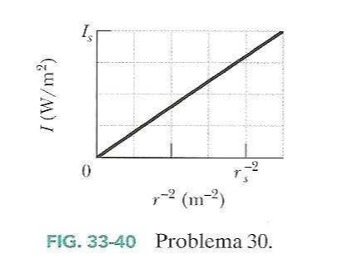
\includegraphics[width=0.45\textwidth]{figures/fig33-40.jpeg}
    \label{fig:33-29}
\end{figure}


\subsubsection{Resolução}
\textbf{Dados}

\[
r = 2,00\,\text{mm} = 2,00\times10^{-3}\,\text{m},
\]

\[
h = 0,500\,\text{m},
\]

\[
\rho = 19,0\,\text{g/cm}^3
      = 1,90\times10^{4}\,\text{kg/m}^3.
\]

A esfera é totalmente absorvente, logo a força de radiação é

\[
F_{\text{rad}}=\frac{IA}{c},
\]

onde \(I\) é a intensidade da radiação na posição da esfera,
\(A=\pi r^2\) é sua área de seção reta e \(c\) é a velocidade da luz.

Para que a esfera fique em equilíbrio,

\[
F_{\text{rad}}=mg.
\]

\bigskip

\textbf{(a) Potência necessária da fonte}

O volume da esfera é

\[
V=\frac{4}{3}\pi r^3,
\]

e sua massa é

\[
m=\rho V
  =\rho\frac{4}{3}\pi r^3.
\]

Substituindo os valores:

\[
m
=(1,90\times10^{4})
\frac{4}{3}\pi(2,00\times10^{-3})^3
\approx 6,37\times10^{-4}\,\text{kg}.
\]

Assim,

\[
mg
=(6,37\times10^{-4})(9,8)
\approx 6,24\times10^{-3}\,\text{N}.
\]

Da condição de equilíbrio,

\[
\frac{I\pi r^2}{c}=mg,
\]

logo

\[
I=\frac{mg\,c}{\pi r^2}.
\]

Substituindo os valores:

\[
I=
\frac{(6,24\times10^{-3})(3,00\times10^{8})}
{\pi(2,00\times10^{-3})^2}
\approx 1,49\times10^{11}\,\text{W/m}^2.
\]

Para uma fonte isotrópica,

\[
I=\frac{P}{4\pi h^2},
\]

portanto

\[
P=4\pi h^2 I.
\]

Com \(h=0,500\,\text{m}\),

\[
P
=4\pi(0,500)^2(1,49\times10^{11})
\approx 4,7\times10^{11}\,\text{W}.
\]

Logo,

\[
\boxed{P \approx 4,7\times10^{11}\ \text{W}}.
\]

\bigskip

\textbf{(b) Estabilidade do equilíbrio}

A intensidade da radiação varia com a distância segundo

\[
I=\frac{P}{4\pi r^2}.
\]

Assim, a força de radiação também varia como

\[
F_{\text{rad}}\propto \frac{1}{r^2}.
\]

Como a força de radiação varia com \(1/r^2\), um pequeno deslocamento altera essa força de modo a afastar ainda mais a esfera da posição de equilíbrio. Portanto, o equilíbrio é

\[
\boxed{\text{instável}}.
\]

\vspace{1cm}
